\documentclass[1p]{elsarticle_modified}
%\bibliographystyle{elsarticle-num}

%\usepackage[colorlinks]{hyperref}
%\usepackage{abbrmath_seonhwa} %\Abb, \Ascr, \Acal ,\Abf, \Afrak
\usepackage{amsfonts}
\usepackage{amssymb}
\usepackage{amsmath}
\usepackage{amsthm}
\usepackage{scalefnt}
\usepackage{amsbsy}
\usepackage{kotex}
\usepackage{caption}
\usepackage{subfig}
\usepackage{color}
\usepackage{graphicx}
\usepackage{xcolor} %% white, black, red, green, blue, cyan, magenta, yellow
\usepackage{float}
\usepackage{setspace}
\usepackage{hyperref}

\usepackage{tikz}
\usetikzlibrary{arrows}

\usepackage{multirow}
\usepackage{array} % fixed length table
\usepackage{hhline}

%%%%%%%%%%%%%%%%%%%%%
\makeatletter
\renewcommand*\env@matrix[1][\arraystretch]{%
	\edef\arraystretch{#1}%
	\hskip -\arraycolsep
	\let\@ifnextchar\new@ifnextchar
	\array{*\c@MaxMatrixCols c}}
\makeatother %https://tex.stackexchange.com/questions/14071/how-can-i-increase-the-line-spacing-in-a-matrix
%%%%%%%%%%%%%%%

\usepackage[normalem]{ulem}

\newcommand{\msout}[1]{\ifmmode\text{\sout{\ensuremath{#1}}}\else\sout{#1}\fi}
%SOURCE: \msout is \stkout macro in https://tex.stackexchange.com/questions/20609/strikeout-in-math-mode

\newcommand{\cancel}[1]{
	\ifmmode
	{\color{red}\msout{#1}}
	\else
	{\color{red}\sout{#1}}
	\fi
}

\newcommand{\add}[1]{
	{\color{blue}\uwave{#1}}
}

\newcommand{\replace}[2]{
	\ifmmode
	{\color{red}\msout{#1}}{\color{blue}\uwave{#2}}
	\else
	{\color{red}\sout{#1}}{\color{blue}\uwave{#2}}
	\fi
}

\newcommand{\Sol}{\mathcal{S}} %segment
\newcommand{\D}{D} %diagram
\newcommand{\A}{\mathcal{A}} %arc


%%%%%%%%%%%%%%%%%%%%%%%%%%%%%5 test

\def\sl{\operatorname{\textup{SL}}(2,\Cbb)}
\def\psl{\operatorname{\textup{PSL}}(2,\Cbb)}
\def\quan{\mkern 1mu \triangleright \mkern 1mu}

\theoremstyle{definition}
\newtheorem{thm}{Theorem}[section]
\newtheorem{prop}[thm]{Proposition}
\newtheorem{lem}[thm]{Lemma}
\newtheorem{ques}[thm]{Question}
\newtheorem{cor}[thm]{Corollary}
\newtheorem{defn}[thm]{Definition}
\newtheorem{exam}[thm]{Example}
\newtheorem{rmk}[thm]{Remark}
\newtheorem{alg}[thm]{Algorithm}

\newcommand{\I}{\sqrt{-1}}
\begin{document}

%\begin{frontmatter}
%
%\title{Boundary parabolic representations of knots up to 8 crossings}
%
%%% Group authors per affiliation:
%\author{Yunhi Cho} 
%\address{Department of Mathematics, University of Seoul, Seoul, Korea}
%\ead{yhcho@uos.ac.kr}
%
%
%\author{Seonhwa Kim} %\fnref{s_kim}}
%\address{Center for Geometry and Physics, Institute for Basic Science, Pohang, 37673, Korea}
%\ead{ryeona17@ibs.re.kr}
%
%\author{Hyuk Kim}
%\address{Department of Mathematical Sciences, Seoul National University, Seoul 08826, Korea}
%\ead{hyukkim@snu.ac.kr}
%
%\author{Seokbeom Yoon}
%\address{Department of Mathematical Sciences, Seoul National University, Seoul, 08826,  Korea}
%\ead{sbyoon15@snu.ac.kr}
%
%\begin{abstract}
%We find all boundary parabolic representation of knots up to 8 crossings.
%
%\end{abstract}
%\begin{keyword}
%    \MSC[2010] 57M25 
%\end{keyword}
%
%\end{frontmatter}

%\linenumbers
%\tableofcontents
%
\newcommand\colored[1]{\textcolor{white}{\rule[-0.35ex]{0.8em}{1.4ex}}\kern-0.8em\color{red} #1}%
%\newcommand\colored[1]{\textcolor{white}{ #1}\kern-2.17ex	\textcolor{white}{ #1}\kern-1.81ex	\textcolor{white}{ #1}\kern-2.15ex\color{red}#1	}

{\Large $\underline{9_{39}~(K9a_{32})}$}

\setlength{\tabcolsep}{10pt}
\renewcommand{\arraystretch}{1.6}
\vspace{1cm}\begin{tabular}{m{100pt}>{\centering\arraybackslash}m{274pt}}
\multirow{5}{120pt}{
	\centering
	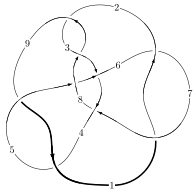
\includegraphics[width=112pt]{../../../GIT/diagram.site/Diagrams/png/74_9_39.png}\\
\ \ \ A knot diagram\footnotemark}&
\allowdisplaybreaks
\textbf{Linearized knot diagam} \\
\cline{2-2}
 &
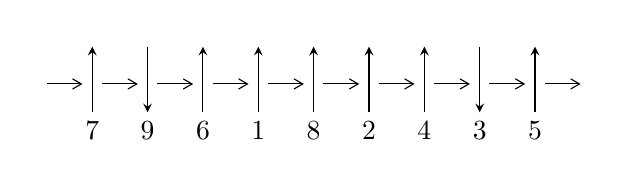
\begin{tikzpicture}[x=20pt, y=17pt]
	% nodes
	\node (C0) at (0, 0) {};
	\node (C1) at (1, 0) {};
	\node (C1U) at (1, +1) {};
	\node (C1D) at (1, -1) {7};

	\node (C2) at (2, 0) {};
	\node (C2U) at (2, +1) {};
	\node (C2D) at (2, -1) {9};

	\node (C3) at (3, 0) {};
	\node (C3U) at (3, +1) {};
	\node (C3D) at (3, -1) {6};

	\node (C4) at (4, 0) {};
	\node (C4U) at (4, +1) {};
	\node (C4D) at (4, -1) {1};

	\node (C5) at (5, 0) {};
	\node (C5U) at (5, +1) {};
	\node (C5D) at (5, -1) {8};

	\node (C6) at (6, 0) {};
	\node (C6U) at (6, +1) {};
	\node (C6D) at (6, -1) {2};

	\node (C7) at (7, 0) {};
	\node (C7U) at (7, +1) {};
	\node (C7D) at (7, -1) {4};

	\node (C8) at (8, 0) {};
	\node (C8U) at (8, +1) {};
	\node (C8D) at (8, -1) {3};

	\node (C9) at (9, 0) {};
	\node (C9U) at (9, +1) {};
	\node (C9D) at (9, -1) {5};
	\node (C10) at (10, 0) {};

	% arrows
	\draw[->,>={angle 60}]
	(C0) edge (C1) (C1) edge (C2) (C2) edge (C3) (C3) edge (C4) (C4) edge (C5) (C5) edge (C6) (C6) edge (C7) (C7) edge (C8) (C8) edge (C9) (C9) edge (C10) ;	\draw[->,>=stealth]
	(C1D) edge (C1U) (C2U) edge (C2D) (C3D) edge (C3U) (C4D) edge (C4U) (C5D) edge (C5U) (C6D) edge (C6U) (C7D) edge (C7U) (C8U) edge (C8D) (C9D) edge (C9U) ;
	\end{tikzpicture} \\
\hhline{~~} \\& 
\textbf{Solving Sequence} \\ \cline{2-2} 
 &
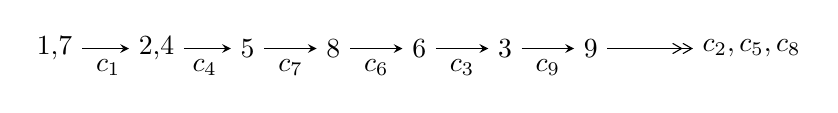
\begin{tikzpicture}[x=31pt, y=7pt]
	% node
	\node (A0) at (-1/8, 0) {1,7};
	\node (A1) at (17/16, 0) {2,4};
	\node (A2) at (17/8, 0) {5};
	\node (A3) at (25/8, 0) {8};
	\node (A4) at (33/8, 0) {6};
	\node (A5) at (41/8, 0) {3};
	\node (A6) at (49/8, 0) {9};
	\node (C1) at (1/2, -1) {$c_{1}$};
	\node (C2) at (13/8, -1) {$c_{4}$};
	\node (C3) at (21/8, -1) {$c_{7}$};
	\node (C4) at (29/8, -1) {$c_{6}$};
	\node (C5) at (37/8, -1) {$c_{3}$};
	\node (C6) at (45/8, -1) {$c_{9}$};
	\node (A7) at (8, 0) {$c_{2},c_{5},c_{8}$};

	% edge
	\draw[->,>=stealth]	
	(A0) edge (A1) (A1) edge (A2) (A2) edge (A3) (A3) edge (A4) (A4) edge (A5) (A5) edge (A6) ;
	\draw[->>,>={angle 60}]	
	(A6) edge (A7);
\end{tikzpicture} \\ 

\end{tabular} \\

\footnotetext{
The image of knot diagram is generated by the software ``\textbf{Draw programme}" developed by Andrew Bartholomew(\url{http://www.layer8.co.uk/maths/draw/index.htm\#Running-draw}), where we modified some parts for our purpose(\url{https://github.com/CATsTAILs/LinksPainter}).
}\phantom \\ \newline 
\centering \textbf{Ideals for irreducible components\footnotemark of $X_{\text{par}}$} 
 
\begin{align*}
I^u_{1}&=\langle 
b- u,\;-17 u^{10}-18 u^9-65 u^8-43 u^7-91 u^6-38 u^5-20 u^4+21 u^3-8 u^2+25 a+10 u-27,\\
\phantom{I^u_{1}}&\phantom{= \langle  }u^{11}+4 u^9- u^8+7 u^7-3 u^6+4 u^5-3 u^4+u^3- u^2+u+1\rangle \\
I^u_{2}&=\langle 
-63269332 u^{19}-195765489 u^{18}+\cdots+599392561 b-259471427,\\
\phantom{I^u_{2}}&\phantom{= \langle  }-102509023 u^{19}-139045747 u^{18}+\cdots+723404815 a-1805214375,\;u^{20}+u^{19}+\cdots-8 u+7\rangle \\
I^u_{3}&=\langle 
b+u,\;- u^3- u^2+a-2 u,\;u^4+2 u^2- u+1\rangle \\
\\
\end{align*}
\raggedright * 3 irreducible components of $\dim_{\mathbb{C}}=0$, with total 35 representations.\\
\footnotetext{All coefficients of polynomials are rational numbers. But the coefficients are sometimes approximated in decimal forms when there is not enough margin.}
\newpage
\renewcommand{\arraystretch}{1}
\centering \section*{I. $I^u_{1}= \langle b- u,\;-17 u^{10}-18 u^9+\cdots+25 a-27,\;u^{11}+4 u^9+\cdots+u+1 \rangle$}
\flushleft \textbf{(i) Arc colorings}\\
\begin{tabular}{m{7pt} m{180pt} m{7pt} m{180pt} }
\flushright $a_{1}=$&$\begin{pmatrix}1\\0\end{pmatrix}$ \\
\flushright $a_{7}=$&$\begin{pmatrix}0\\u\end{pmatrix}$ \\
\flushright $a_{2}=$&$\begin{pmatrix}1\\- u^2\end{pmatrix}$ \\
\flushright $a_{4}=$&$\begin{pmatrix}0.680000 u^{10}+0.720000 u^{9}+\cdots-0.400000 u+1.08000\\u\end{pmatrix}$ \\
\flushright $a_{5}=$&$\begin{pmatrix}0.680000 u^{10}+0.720000 u^{9}+\cdots+0.600000 u+1.08000\\u\end{pmatrix}$ \\
\flushright $a_{8}=$&$\begin{pmatrix}-0.320000 u^{10}-1.28000 u^{9}+\cdots-0.400000 u-0.920000\\-0.120000 u^{10}-0.480000 u^{9}+\cdots-0.400000 u-0.720000\end{pmatrix}$ \\
\flushright $a_{6}=$&$\begin{pmatrix}- u\\u^3+u\end{pmatrix}$ \\
\flushright $a_{3}=$&$\begin{pmatrix}0.720000 u^{10}+0.880000 u^{9}+\cdots+0.400000 u+1.32000\\\frac{8}{25} u^{10}+\frac{7}{25} u^9+\cdots+\frac{2}{5} u-\frac{2}{25}\end{pmatrix}$ \\
\flushright $a_{9}=$&$\begin{pmatrix}\frac{18}{25} u^{10}-\frac{3}{25} u^9+\cdots+\frac{2}{5} u+\frac{8}{25}\\u^2\end{pmatrix}$\\ \flushright $a_{9}=$&$\begin{pmatrix}\frac{18}{25} u^{10}-\frac{3}{25} u^9+\cdots+\frac{2}{5} u+\frac{8}{25}\\u^2\end{pmatrix}$\\&\end{tabular}
\flushleft \textbf{(ii) Obstruction class $= -1$}\\~\\
\flushleft \textbf{(iii) Cusp Shapes $= \frac{31}{25} u^{10}-\frac{51}{25} u^9+\frac{24}{5} u^8-\frac{201}{25} u^7+\frac{238}{25} u^6-\frac{341}{25} u^5+\frac{47}{5} u^4-\frac{103}{25} u^3+\frac{144}{25} u^2-\frac{6}{5} u+\frac{211}{25}$}\\~\\
\newpage\renewcommand{\arraystretch}{1}
\flushleft \textbf{(iv) u-Polynomials at the component}\newline \\
\begin{tabular}{m{50pt}|m{274pt}}
Crossings & \hspace{64pt}u-Polynomials at each crossing \\
\hline $$\begin{aligned}c_{1},c_{4},c_{6}\\c_{9}\end{aligned}$$&$\begin{aligned}
&u^{11}+4 u^9+u^8+7 u^7+3 u^6+4 u^5+3 u^4+u^3+u^2+u-1
\end{aligned}$\\
\hline $$\begin{aligned}c_{2},c_{8}\end{aligned}$$&$\begin{aligned}
&u^{11}-6 u^{10}+\cdots+26 u-4
\end{aligned}$\\
\hline $$\begin{aligned}c_{3},c_{5}\end{aligned}$$&$\begin{aligned}
&u^{11}-2 u^9-3 u^8+7 u^7+3 u^6-4 u^5-9 u^4+5 u^3+5 u^2- u-1
\end{aligned}$\\
\hline $$\begin{aligned}c_{7}\end{aligned}$$&$\begin{aligned}
&u^{11}-10 u^{10}+\cdots+176 u-32
\end{aligned}$\\
\hline
\end{tabular}\\~\\
\newpage\renewcommand{\arraystretch}{1}
\flushleft \textbf{(v) Riley Polynomials at the component}\newline \\
\begin{tabular}{m{50pt}|m{274pt}}
Crossings & \hspace{64pt}Riley Polynomials at each crossing \\
\hline $$\begin{aligned}c_{1},c_{4},c_{6}\\c_{9}\end{aligned}$$&$\begin{aligned}
&y^{11}+8 y^{10}+\cdots+3 y-1
\end{aligned}$\\
\hline $$\begin{aligned}c_{2},c_{8}\end{aligned}$$&$\begin{aligned}
&y^{11}+6 y^{10}+\cdots+124 y-16
\end{aligned}$\\
\hline $$\begin{aligned}c_{3},c_{5}\end{aligned}$$&$\begin{aligned}
&y^{11}-4 y^{10}+\cdots+11 y-1
\end{aligned}$\\
\hline $$\begin{aligned}c_{7}\end{aligned}$$&$\begin{aligned}
&y^{11}+2 y^9+\cdots+1792 y-1024
\end{aligned}$\\
\hline
\end{tabular}\\~\\
\newpage\flushleft \textbf{(vi) Complex Volumes and Cusp Shapes}
$$\begin{array}{c|c|c}  
\text{Solutions to }I^u_{1}& \I (\text{vol} + \sqrt{-1}CS) & \text{Cusp shape}\\
 \hline 
\begin{aligned}
u &= \phantom{-}0.127465 + 1.057020 I \\
a &= \phantom{-}0.26477 + 1.83548 I \\
b &= \phantom{-}0.127465 + 1.057020 I\end{aligned}
 & -0.55548 + 3.69188 I & \phantom{-}3.27466 - 4.59532 I \\ \hline\begin{aligned}
u &= \phantom{-}0.127465 - 1.057020 I \\
a &= \phantom{-}0.26477 - 1.83548 I \\
b &= \phantom{-}0.127465 - 1.057020 I\end{aligned}
 & -0.55548 - 3.69188 I & \phantom{-}3.27466 + 4.59532 I \\ \hline\begin{aligned}
u &= -0.483399 + 0.706724 I \\
a &= \phantom{-}1.104400 - 0.699054 I \\
b &= -0.483399 + 0.706724 I\end{aligned}
 & \phantom{-}1.11176 - 2.13095 I & \phantom{-}7.34122 + 2.95650 I \\ \hline\begin{aligned}
u &= -0.483399 - 0.706724 I \\
a &= \phantom{-}1.104400 + 0.699054 I \\
b &= -0.483399 - 0.706724 I\end{aligned}
 & \phantom{-}1.11176 + 2.13095 I & \phantom{-}7.34122 - 2.95650 I \\ \hline\begin{aligned}
u &= \phantom{-}0.726207 + 0.303425 I \\
a &= -0.834499 + 0.996603 I \\
b &= \phantom{-}0.726207 + 0.303425 I\end{aligned}
 & \phantom{-}3.57861 - 2.27941 I & \phantom{-}10.11894 + 1.15857 I \\ \hline\begin{aligned}
u &= \phantom{-}0.726207 - 0.303425 I \\
a &= -0.834499 - 0.996603 I \\
b &= \phantom{-}0.726207 - 0.303425 I\end{aligned}
 & \phantom{-}3.57861 + 2.27941 I & \phantom{-}10.11894 - 1.15857 I \\ \hline\begin{aligned}
u &= \phantom{-}0.424463 + 1.293840 I \\
a &= -1.334040 + 0.269858 I \\
b &= \phantom{-}0.424463 + 1.293840 I\end{aligned}
 & -6.69869 + 6.38540 I & \phantom{-}0.12486 - 5.46357 I \\ \hline\begin{aligned}
u &= \phantom{-}0.424463 - 1.293840 I \\
a &= -1.334040 - 0.269858 I \\
b &= \phantom{-}0.424463 - 1.293840 I\end{aligned}
 & -6.69869 - 6.38540 I & \phantom{-}0.12486 + 5.46357 I \\ \hline\begin{aligned}
u &= -0.56939 + 1.41435 I \\
a &= \phantom{-}1.081850 + 0.205459 I \\
b &= -0.56939 + 1.41435 I\end{aligned}
 & -3.64137 - 12.81030 I & \phantom{-}2.99547 + 7.42806 I \\ \hline\begin{aligned}
u &= -0.56939 - 1.41435 I \\
a &= \phantom{-}1.081850 - 0.205459 I \\
b &= -0.56939 - 1.41435 I\end{aligned}
 & -3.64137 + 12.81030 I & \phantom{-}2.99547 - 7.42806 I\\
 \hline 
 \end{array}$$\newpage$$\begin{array}{c|c|c}  
\text{Solutions to }I^u_{1}& \I (\text{vol} + \sqrt{-1}CS) & \text{Cusp shape}\\
 \hline 
\begin{aligned}
u &= -0.450687\phantom{ +0.000000I} \\
a &= \phantom{-}1.43503\phantom{ +0.000000I} \\
b &= -0.450687\phantom{ +0.000000I}\end{aligned}
 & \phantom{-}0.895812\phantom{ +0.000000I} & \phantom{-}11.2900\phantom{ +0.000000I}\\
 \hline 
 \end{array}$$\newpage\newpage\renewcommand{\arraystretch}{1}
\centering \section*{II. $I^u_{2}= \langle -6.33\times10^{7} u^{19}-1.96\times10^{8} u^{18}+\cdots+5.99\times10^{8} b-2.59\times10^{8},\;-1.03\times10^{8} u^{19}-1.39\times10^{8} u^{18}+\cdots+7.23\times10^{8} a-1.81\times10^{9},\;u^{20}+u^{19}+\cdots-8 u+7 \rangle$}
\flushleft \textbf{(i) Arc colorings}\\
\begin{tabular}{m{7pt} m{180pt} m{7pt} m{180pt} }
\flushright $a_{1}=$&$\begin{pmatrix}1\\0\end{pmatrix}$ \\
\flushright $a_{7}=$&$\begin{pmatrix}0\\u\end{pmatrix}$ \\
\flushright $a_{2}=$&$\begin{pmatrix}1\\- u^2\end{pmatrix}$ \\
\flushright $a_{4}=$&$\begin{pmatrix}0.141704 u^{19}+0.192210 u^{18}+\cdots-2.03306 u+2.49544\\0.105556 u^{19}+0.326606 u^{18}+\cdots+1.69754 u+0.432891\end{pmatrix}$ \\
\flushright $a_{5}=$&$\begin{pmatrix}0.247259 u^{19}+0.518817 u^{18}+\cdots-0.335520 u+2.92833\\0.105556 u^{19}+0.326606 u^{18}+\cdots+1.69754 u+0.432891\end{pmatrix}$ \\
\flushright $a_{8}=$&$\begin{pmatrix}0.284561 u^{19}+0.335067 u^{18}+\cdots+3.39551 u+1.35258\\0.164678 u^{19}+0.105389 u^{18}+\cdots+3.03699 u-1.41642\end{pmatrix}$ \\
\flushright $a_{6}=$&$\begin{pmatrix}- u\\u^3+u\end{pmatrix}$ \\
\flushright $a_{3}=$&$\begin{pmatrix}0.149091 u^{19}+0.564154 u^{18}+\cdots-4.13459 u+4.66739\\0.109222 u^{19}+0.420500 u^{18}+\cdots+0.934319 u+0.812840\end{pmatrix}$ \\
\flushright $a_{9}=$&$\begin{pmatrix}-0.349552 u^{19}-0.0796380 u^{18}+\cdots-1.25873 u+1.73518\\-0.551898 u^{19}-0.446663 u^{18}+\cdots-6.28274 u+0.316957\end{pmatrix}$\\ \flushright $a_{9}=$&$\begin{pmatrix}-0.349552 u^{19}-0.0796380 u^{18}+\cdots-1.25873 u+1.73518\\-0.551898 u^{19}-0.446663 u^{18}+\cdots-6.28274 u+0.316957\end{pmatrix}$\\&\end{tabular}
\flushleft \textbf{(ii) Obstruction class $= -1$}\\~\\
\flushleft \textbf{(iii) Cusp Shapes $= -\frac{1402773924}{2996962805} u^{19}-\frac{100220208}{2996962805} u^{18}+\cdots-\frac{22381283924}{2996962805} u+\frac{26005127826}{2996962805}$}\\~\\
\newpage\renewcommand{\arraystretch}{1}
\flushleft \textbf{(iv) u-Polynomials at the component}\newline \\
\begin{tabular}{m{50pt}|m{274pt}}
Crossings & \hspace{64pt}u-Polynomials at each crossing \\
\hline $$\begin{aligned}c_{1},c_{4},c_{6}\\c_{9}\end{aligned}$$&$\begin{aligned}
&u^{20}- u^{19}+\cdots+8 u+7
\end{aligned}$\\
\hline $$\begin{aligned}c_{2},c_{8}\end{aligned}$$&$\begin{aligned}
&(u^5+u^4+2 u^3+u^2+u+1)^4
\end{aligned}$\\
\hline $$\begin{aligned}c_{3},c_{5}\end{aligned}$$&$\begin{aligned}
&u^{20}+5 u^{19}+\cdots+2 u+1
\end{aligned}$\\
\hline $$\begin{aligned}c_{7}\end{aligned}$$&$\begin{aligned}
&(u^2+u+1)^{10}
\end{aligned}$\\
\hline
\end{tabular}\\~\\
\newpage\renewcommand{\arraystretch}{1}
\flushleft \textbf{(v) Riley Polynomials at the component}\newline \\
\begin{tabular}{m{50pt}|m{274pt}}
Crossings & \hspace{64pt}Riley Polynomials at each crossing \\
\hline $$\begin{aligned}c_{1},c_{4},c_{6}\\c_{9}\end{aligned}$$&$\begin{aligned}
&y^{20}+15 y^{19}+\cdots+468 y+49
\end{aligned}$\\
\hline $$\begin{aligned}c_{2},c_{8}\end{aligned}$$&$\begin{aligned}
&(y^5+3 y^4+4 y^3+y^2- y-1)^4
\end{aligned}$\\
\hline $$\begin{aligned}c_{3},c_{5}\end{aligned}$$&$\begin{aligned}
&y^{20}+3 y^{19}+\cdots+12 y+1
\end{aligned}$\\
\hline $$\begin{aligned}c_{7}\end{aligned}$$&$\begin{aligned}
&(y^2+y+1)^{10}
\end{aligned}$\\
\hline
\end{tabular}\\~\\
\newpage\flushleft \textbf{(vi) Complex Volumes and Cusp Shapes}
$$\begin{array}{c|c|c}  
\text{Solutions to }I^u_{2}& \I (\text{vol} + \sqrt{-1}CS) & \text{Cusp shape}\\
 \hline 
\begin{aligned}
u &= -0.590252 + 0.825819 I \\
a &= \phantom{-}0.407671 - 0.896841 I \\
b &= \phantom{-}0.070663 + 0.512466 I\end{aligned}
 & \phantom{-}0.93776 - 2.37095 I & \phantom{-}4.74431 + 0.03448 I \\ \hline\begin{aligned}
u &= -0.590252 - 0.825819 I \\
a &= \phantom{-}0.407671 + 0.896841 I \\
b &= \phantom{-}0.070663 - 0.512466 I\end{aligned}
 & \phantom{-}0.93776 + 2.37095 I & \phantom{-}4.74431 - 0.03448 I \\ \hline\begin{aligned}
u &= \phantom{-}0.067213 + 1.072300 I \\
a &= \phantom{-}0.833585 - 0.414037 I \\
b &= -0.38849 - 1.61565 I\end{aligned}
 & -4.60570 + 0.49930 I & \phantom{-}0.515115 + 0.966547 I \\ \hline\begin{aligned}
u &= \phantom{-}0.067213 - 1.072300 I \\
a &= \phantom{-}0.833585 + 0.414037 I \\
b &= -0.38849 + 1.61565 I\end{aligned}
 & -4.60570 - 0.49930 I & \phantom{-}0.515115 - 0.966547 I \\ \hline\begin{aligned}
u &= -0.130820 + 1.153330 I \\
a &= -0.789899 - 0.343929 I \\
b &= \phantom{-}0.739688 - 0.098744 I\end{aligned}
 & -2.53372 - 2.02988 I & \phantom{-}1.48114 + 3.46410 I \\ \hline\begin{aligned}
u &= -0.130820 - 1.153330 I \\
a &= -0.789899 + 0.343929 I \\
b &= \phantom{-}0.739688 + 0.098744 I\end{aligned}
 & -2.53372 + 2.02988 I & \phantom{-}1.48114 - 3.46410 I \\ \hline\begin{aligned}
u &= \phantom{-}0.387179 + 1.147990 I \\
a &= \phantom{-}0.809229 - 0.162618 I \\
b &= -1.286370 - 0.028870 I\end{aligned}
 & \phantom{-}0.93776 + 6.43072 I & \phantom{-}4.74431 - 6.96269 I \\ \hline\begin{aligned}
u &= \phantom{-}0.387179 - 1.147990 I \\
a &= \phantom{-}0.809229 + 0.162618 I \\
b &= -1.286370 + 0.028870 I\end{aligned}
 & \phantom{-}0.93776 - 6.43072 I & \phantom{-}4.74431 + 6.96269 I \\ \hline\begin{aligned}
u &= \phantom{-}0.739688 + 0.098744 I \\
a &= \phantom{-}0.817684 + 1.061640 I \\
b &= -0.130820 - 1.153330 I\end{aligned}
 & -2.53372 + 2.02988 I & \phantom{-}1.48114 - 3.46410 I \\ \hline\begin{aligned}
u &= \phantom{-}0.739688 - 0.098744 I \\
a &= \phantom{-}0.817684 - 1.061640 I \\
b &= -0.130820 + 1.153330 I\end{aligned}
 & -2.53372 - 2.02988 I & \phantom{-}1.48114 + 3.46410 I\\
 \hline 
 \end{array}$$\newpage$$\begin{array}{c|c|c}  
\text{Solutions to }I^u_{2}& \I (\text{vol} + \sqrt{-1}CS) & \text{Cusp shape}\\
 \hline 
\begin{aligned}
u &= -1.286370 + 0.028870 I \\
a &= -0.403596 + 0.664172 I \\
b &= \phantom{-}0.387179 - 1.147990 I\end{aligned}
 & \phantom{-}0.93776 - 6.43072 I & \phantom{-}4.74431 + 6.96269 I \\ \hline\begin{aligned}
u &= -1.286370 - 0.028870 I \\
a &= -0.403596 - 0.664172 I \\
b &= \phantom{-}0.387179 + 1.147990 I\end{aligned}
 & \phantom{-}0.93776 + 6.43072 I & \phantom{-}4.74431 - 6.96269 I \\ \hline\begin{aligned}
u &= -0.133857 + 1.341630 I \\
a &= -0.675959 - 0.305240 I \\
b &= \phantom{-}0.76505 - 1.34819 I\end{aligned}
 & -4.60570 - 3.56046 I & \phantom{-}0.51511 + 7.89475 I \\ \hline\begin{aligned}
u &= -0.133857 - 1.341630 I \\
a &= -0.675959 + 0.305240 I \\
b &= \phantom{-}0.76505 + 1.34819 I\end{aligned}
 & -4.60570 + 3.56046 I & \phantom{-}0.51511 - 7.89475 I \\ \hline\begin{aligned}
u &= \phantom{-}0.070663 + 0.512466 I \\
a &= \phantom{-}1.79041 - 0.72880 I \\
b &= -0.590252 + 0.825819 I\end{aligned}
 & \phantom{-}0.93776 - 2.37095 I & \phantom{-}4.74431 + 0.03448 I \\ \hline\begin{aligned}
u &= \phantom{-}0.070663 - 0.512466 I \\
a &= \phantom{-}1.79041 + 0.72880 I \\
b &= -0.590252 - 0.825819 I\end{aligned}
 & \phantom{-}0.93776 + 2.37095 I & \phantom{-}4.74431 - 0.03448 I \\ \hline\begin{aligned}
u &= \phantom{-}0.76505 + 1.34819 I \\
a &= \phantom{-}0.645088 - 0.004802 I \\
b &= -0.133857 - 1.341630 I\end{aligned}
 & -4.60570 + 3.56046 I & \phantom{-}0.51511 - 7.89475 I \\ \hline\begin{aligned}
u &= \phantom{-}0.76505 - 1.34819 I \\
a &= \phantom{-}0.645088 + 0.004802 I \\
b &= -0.133857 + 1.341630 I\end{aligned}
 & -4.60570 - 3.56046 I & \phantom{-}0.51511 + 7.89475 I \\ \hline\begin{aligned}
u &= -0.38849 + 1.61565 I \\
a &= -0.577071 - 0.170713 I \\
b &= \phantom{-}0.067213 - 1.072300 I\end{aligned}
 & -4.60570 - 0.49930 I & \phantom{-}0.515115 - 0.966547 I \\ \hline\begin{aligned}
u &= -0.38849 - 1.61565 I \\
a &= -0.577071 + 0.170713 I \\
b &= \phantom{-}0.067213 + 1.072300 I\end{aligned}
 & -4.60570 + 0.49930 I & \phantom{-}0.515115 + 0.966547 I\\
 \hline 
 \end{array}$$\newpage\newpage\renewcommand{\arraystretch}{1}
\centering \section*{III. $I^u_{3}= \langle b+u,\;- u^3- u^2+a-2 u,\;u^4+2 u^2- u+1 \rangle$}
\flushleft \textbf{(i) Arc colorings}\\
\begin{tabular}{m{7pt} m{180pt} m{7pt} m{180pt} }
\flushright $a_{1}=$&$\begin{pmatrix}1\\0\end{pmatrix}$ \\
\flushright $a_{7}=$&$\begin{pmatrix}0\\u\end{pmatrix}$ \\
\flushright $a_{2}=$&$\begin{pmatrix}1\\- u^2\end{pmatrix}$ \\
\flushright $a_{4}=$&$\begin{pmatrix}u^3+u^2+2 u\\- u\end{pmatrix}$ \\
\flushright $a_{5}=$&$\begin{pmatrix}u^3+u^2+u\\- u\end{pmatrix}$ \\
\flushright $a_{8}=$&$\begin{pmatrix}- u^3- u^2-2 u-1\\u^2+u+1\end{pmatrix}$ \\
\flushright $a_{6}=$&$\begin{pmatrix}- u\\u^3+u\end{pmatrix}$ \\
\flushright $a_{3}=$&$\begin{pmatrix}2 u^3+u^2+3 u\\- u^2- u\end{pmatrix}$ \\
\flushright $a_{9}=$&$\begin{pmatrix}- u^3+u^2- u+2\\u^2\end{pmatrix}$\\ \flushright $a_{9}=$&$\begin{pmatrix}- u^3+u^2- u+2\\u^2\end{pmatrix}$\\&\end{tabular}
\flushleft \textbf{(ii) Obstruction class $= 1$}\\~\\
\flushleft \textbf{(iii) Cusp Shapes $= -7 u^3-2 u^2-11 u+8$}\\~\\
\newpage\renewcommand{\arraystretch}{1}
\flushleft \textbf{(iv) u-Polynomials at the component}\newline \\
\begin{tabular}{m{50pt}|m{274pt}}
Crossings & \hspace{64pt}u-Polynomials at each crossing \\
\hline $$\begin{aligned}c_{1},c_{4}\end{aligned}$$&$\begin{aligned}
&u^4+2 u^2- u+1
\end{aligned}$\\
\hline $$\begin{aligned}c_{2}\end{aligned}$$&$\begin{aligned}
&u^4+u^3+2 u^2+1
\end{aligned}$\\
\hline $$\begin{aligned}c_{3},c_{5}\end{aligned}$$&$\begin{aligned}
&u^4+u+1
\end{aligned}$\\
\hline $$\begin{aligned}c_{6},c_{9}\end{aligned}$$&$\begin{aligned}
&u^4+2 u^2+u+1
\end{aligned}$\\
\hline $$\begin{aligned}c_{7}\end{aligned}$$&$\begin{aligned}
&u^4- u^3+1
\end{aligned}$\\
\hline $$\begin{aligned}c_{8}\end{aligned}$$&$\begin{aligned}
&u^4- u^3+2 u^2+1
\end{aligned}$\\
\hline
\end{tabular}\\~\\
\newpage\renewcommand{\arraystretch}{1}
\flushleft \textbf{(v) Riley Polynomials at the component}\newline \\
\begin{tabular}{m{50pt}|m{274pt}}
Crossings & \hspace{64pt}Riley Polynomials at each crossing \\
\hline $$\begin{aligned}c_{1},c_{4},c_{6}\\c_{9}\end{aligned}$$&$\begin{aligned}
&y^4+4 y^3+6 y^2+3 y+1
\end{aligned}$\\
\hline $$\begin{aligned}c_{2},c_{8}\end{aligned}$$&$\begin{aligned}
&y^4+3 y^3+6 y^2+4 y+1
\end{aligned}$\\
\hline $$\begin{aligned}c_{3},c_{5}\end{aligned}$$&$\begin{aligned}
&y^4+2 y^2- y+1
\end{aligned}$\\
\hline $$\begin{aligned}c_{7}\end{aligned}$$&$\begin{aligned}
&y^4- y^3+2 y^2+1
\end{aligned}$\\
\hline
\end{tabular}\\~\\
\newpage\flushleft \textbf{(vi) Complex Volumes and Cusp Shapes}
$$\begin{array}{c|c|c}  
\text{Solutions to }I^u_{3}& \I (\text{vol} + \sqrt{-1}CS) & \text{Cusp shape}\\
 \hline 
\begin{aligned}
u &= \phantom{-}0.343815 + 0.625358 I \\
a &= \phantom{-}0.05204 + 1.65794 I \\
b &= -0.343815 - 0.625358 I\end{aligned}
 & \phantom{-}1.13814 + 3.38562 I & \phantom{-}7.30286 - 7.57942 I \\ \hline\begin{aligned}
u &= \phantom{-}0.343815 - 0.625358 I \\
a &= \phantom{-}0.05204 - 1.65794 I \\
b &= -0.343815 + 0.625358 I\end{aligned}
 & \phantom{-}1.13814 - 3.38562 I & \phantom{-}7.30286 + 7.57942 I \\ \hline\begin{aligned}
u &= -0.343815 + 1.358440 I \\
a &= -0.552038 - 0.242275 I \\
b &= \phantom{-}0.343815 - 1.358440 I\end{aligned}
 & -4.42801 - 2.37936 I & \phantom{-}2.19714 + 1.10073 I \\ \hline\begin{aligned}
u &= -0.343815 - 1.358440 I \\
a &= -0.552038 + 0.242275 I \\
b &= \phantom{-}0.343815 + 1.358440 I\end{aligned}
 & -4.42801 + 2.37936 I & \phantom{-}2.19714 - 1.10073 I\\
 \hline 
 \end{array}$$\newpage
\newpage\renewcommand{\arraystretch}{1}
\centering \section*{ IV. u-Polynomials}
\begin{tabular}{m{50pt}|m{274pt}}
Crossings & \hspace{64pt}u-Polynomials at each crossing \\
\hline $$\begin{aligned}c_{1},c_{4}\end{aligned}$$&$\begin{aligned}
&(u^4+2 u^2- u+1)\\
&\cdot(u^{11}+4 u^9+u^8+7 u^7+3 u^6+4 u^5+3 u^4+u^3+u^2+u-1)\\
&\cdot(u^{20}- u^{19}+\cdots+8 u+7)
\end{aligned}$\\
\hline $$\begin{aligned}c_{2}\end{aligned}$$&$\begin{aligned}
&(u^4+u^3+2 u^2+1)(u^5+u^4+2 u^3+u^2+u+1)^4\\
&\cdot(u^{11}-6 u^{10}+\cdots+26 u-4)
\end{aligned}$\\
\hline $$\begin{aligned}c_{3},c_{5}\end{aligned}$$&$\begin{aligned}
&(u^4+u+1)(u^{11}-2 u^9+\cdots- u-1)\\
&\cdot(u^{20}+5 u^{19}+\cdots+2 u+1)
\end{aligned}$\\
\hline $$\begin{aligned}c_{6},c_{9}\end{aligned}$$&$\begin{aligned}
&(u^4+2 u^2+u+1)\\
&\cdot(u^{11}+4 u^9+u^8+7 u^7+3 u^6+4 u^5+3 u^4+u^3+u^2+u-1)\\
&\cdot(u^{20}- u^{19}+\cdots+8 u+7)
\end{aligned}$\\
\hline $$\begin{aligned}c_{7}\end{aligned}$$&$\begin{aligned}
&((u^2+u+1)^{10})(u^4- u^3+1)(u^{11}-10 u^{10}+\cdots+176 u-32)
\end{aligned}$\\
\hline $$\begin{aligned}c_{8}\end{aligned}$$&$\begin{aligned}
&(u^4- u^3+2 u^2+1)(u^5+u^4+2 u^3+u^2+u+1)^4\\
&\cdot(u^{11}-6 u^{10}+\cdots+26 u-4)
\end{aligned}$\\
\hline
\end{tabular}\newpage\renewcommand{\arraystretch}{1}
\centering \section*{ V. Riley Polynomials}
\begin{tabular}{m{50pt}|m{274pt}}
Crossings & \hspace{64pt}Riley Polynomials at each crossing \\
\hline $$\begin{aligned}c_{1},c_{4},c_{6}\\c_{9}\end{aligned}$$&$\begin{aligned}
&(y^4+4 y^3+6 y^2+3 y+1)(y^{11}+8 y^{10}+\cdots+3 y-1)\\
&\cdot(y^{20}+15 y^{19}+\cdots+468 y+49)
\end{aligned}$\\
\hline $$\begin{aligned}c_{2},c_{8}\end{aligned}$$&$\begin{aligned}
&(y^4+3 y^3+6 y^2+4 y+1)(y^5+3 y^4+4 y^3+y^2- y-1)^4\\
&\cdot(y^{11}+6 y^{10}+\cdots+124 y-16)
\end{aligned}$\\
\hline $$\begin{aligned}c_{3},c_{5}\end{aligned}$$&$\begin{aligned}
&(y^4+2 y^2- y+1)(y^{11}-4 y^{10}+\cdots+11 y-1)\\
&\cdot(y^{20}+3 y^{19}+\cdots+12 y+1)
\end{aligned}$\\
\hline $$\begin{aligned}c_{7}\end{aligned}$$&$\begin{aligned}
&((y^2+y+1)^{10})(y^4- y^3+2 y^2+1)(y^{11}+2 y^{9}+\cdots+1792 y-1024)
\end{aligned}$\\
\hline
\end{tabular}
\vskip 2pc
\end{document}